\documentclass[12pt]{report}
\usepackage[margin=1in]{geometry}
\usepackage{amsmath,amsthm,amssymb}
\usepackage{graphicx}
\graphicspath{ {images/} }
 
\newcommand{\N}{\mathbb{N}}
\newcommand{\Z}{\mathbb{Z}}
\newcommand{\R}{\mathbb{R}}
\newcommand{\Indicator}{\mathds{1}}
\newcommand{\EX}{\mathbb{E}}
\newcommand{\Prob}{\mathbb{P}}

\begin{document}

\section*{Minimizing the Expectations}

\subsection*{The Balanced Loss Function}

To compute the balanced policy, the following equation must be minimized.

$$
	g_s(q_s^B) = \max\{l_s^B(q_s), \pi_s^B(q_s)\}
$$
where $l_s^B(q_s), \pi_s^B(q_s)$ are as they were defined previously. For general distributions, these equations can be difficult to solve. However, assuming the demand has a multivariate normal distribution, there is a closed form solution.  

\subsubsection*{Holding Function $l_s^B(q_s)$}

Unfortunately, $l_s^B(q_s)$ is the result of a $T - s$ dimensional integral, but it can be reduced a series of $T-s$ integrals of 1 dimension, where the later terms of the series are small. Letting $\Phi_{f_s}$ be the distribution of forecast $f_s$: 
\begin{alignat*}{1}
	l_s^B(q_s) &= \EX [H_s^B(q_s) \; | \; f_s] \\
        &= \EX \bigg\{\sum_{j=s}^T h_j\bigg[q_s - \bigg(\sum_{i=s}^j u_i - X_s\bigg)^+\bigg]^+  \; | \; f_s \bigg\} \\
		&= \int_{u_s}^{\infty} \int_{u_{(s+1)}}^{\infty}\dots \int_{u_T}^{\infty}\sum_{j=s}^T h_j\bigg[q_s - \bigg(\sum_{i=s}^j u_i - X_s\bigg)^+\bigg]^+ d\Phi(u_s, u_{s+1}, \dots u_T)\\
	   &= \sum_{j=s}^T \int_{u_s}^{\infty} \int_{u_{(s+1)}}^{\infty}\dots \int_{u_j}^{\infty} h_j\bigg[q_s - \bigg(\sum_{i=s}^j u_i - X_s\bigg)^+\bigg]^+ d\Phi(u_s, u_{s+1}, \dots u_T)
\end{alignat*}
Given the assumption that the demands are multivariate normal, and letting $D_{[s, j]} = \sum_{i=s}^j D_s$, $D_{[s, j]} \sim N(\sum_{i=s}^j \mu_i, \sum_{i=s}^j \sigma_i^2)$, the expectation can be written as the sum of $(T - s)$ integrals. 
\begin{equation}
	l_s^B(q_s) = \sum_{j=s}^T \int_{u_j=X_s}^{X_s + q_s} h_j\bigg(q_s + X_s - u_j \bigg) d\Phi(u_j)
\end{equation}
It's worth noting that for any individual sample path, there will be a period for which all periods beyond it have 0 holding cost. For simulated solutions, this can be immediately utilized as a stopping rule. For analytical solutions, this could be used for a further approximation (generalizing between the myopic and horizon forms). 

This function has the following derivative.
\begin{alignat*}{1}
	\frac{d}{d q_s} l_s^B(q_s) &=  \sum_{j=s}^T \int_{u_j=X_s}^{X_s + q_s} h_j d\Phi(u_j) \\
		&=  \sum_{j=s}^T h_j (\Phi(X_s + q_s) - \Phi(X_s)) \\
\end{alignat*}

\subsubsection*{Penalty Function $\pi_s^B(q_s)$}

$\pi_s^B(q_s)$ is a more manageable integral.
\begin{alignat}{1}
	\pi_s^B(q_s) &= \EX [\Pi_t^B(q_s) \; | \; f_s] \nonumber \\
		&= \EX \bigg\{ p_s [D_s - (X_s^B + q_s)]^+  \; | \; f_s \bigg\} \nonumber \\
		&= \int_{u_s=({X_s^B + q_s})}^{\infty} p_s (u_s - X_s^B - q_s) d\Phi_s(u_s) 
\end{alignat}

This function has the following derivative.
\begin{alignat*}{1}
	\frac{d}{d q_s} \pi_s^B(q_s) &=  - \int_{u_s=({X_s^B + q_s})}^{\infty} p_s d\Phi_s(u_s) \\
		&= - p_s (1 - \Phi_s(X_s^B + q_s)) 
\end{alignat*}

\subsubsection*{Loss Function}

As an informal validation, the loss function was computed exactly, and using simulated results with 100 replicates. An arbitrary scenario was picked for this task. The results are plotted below:

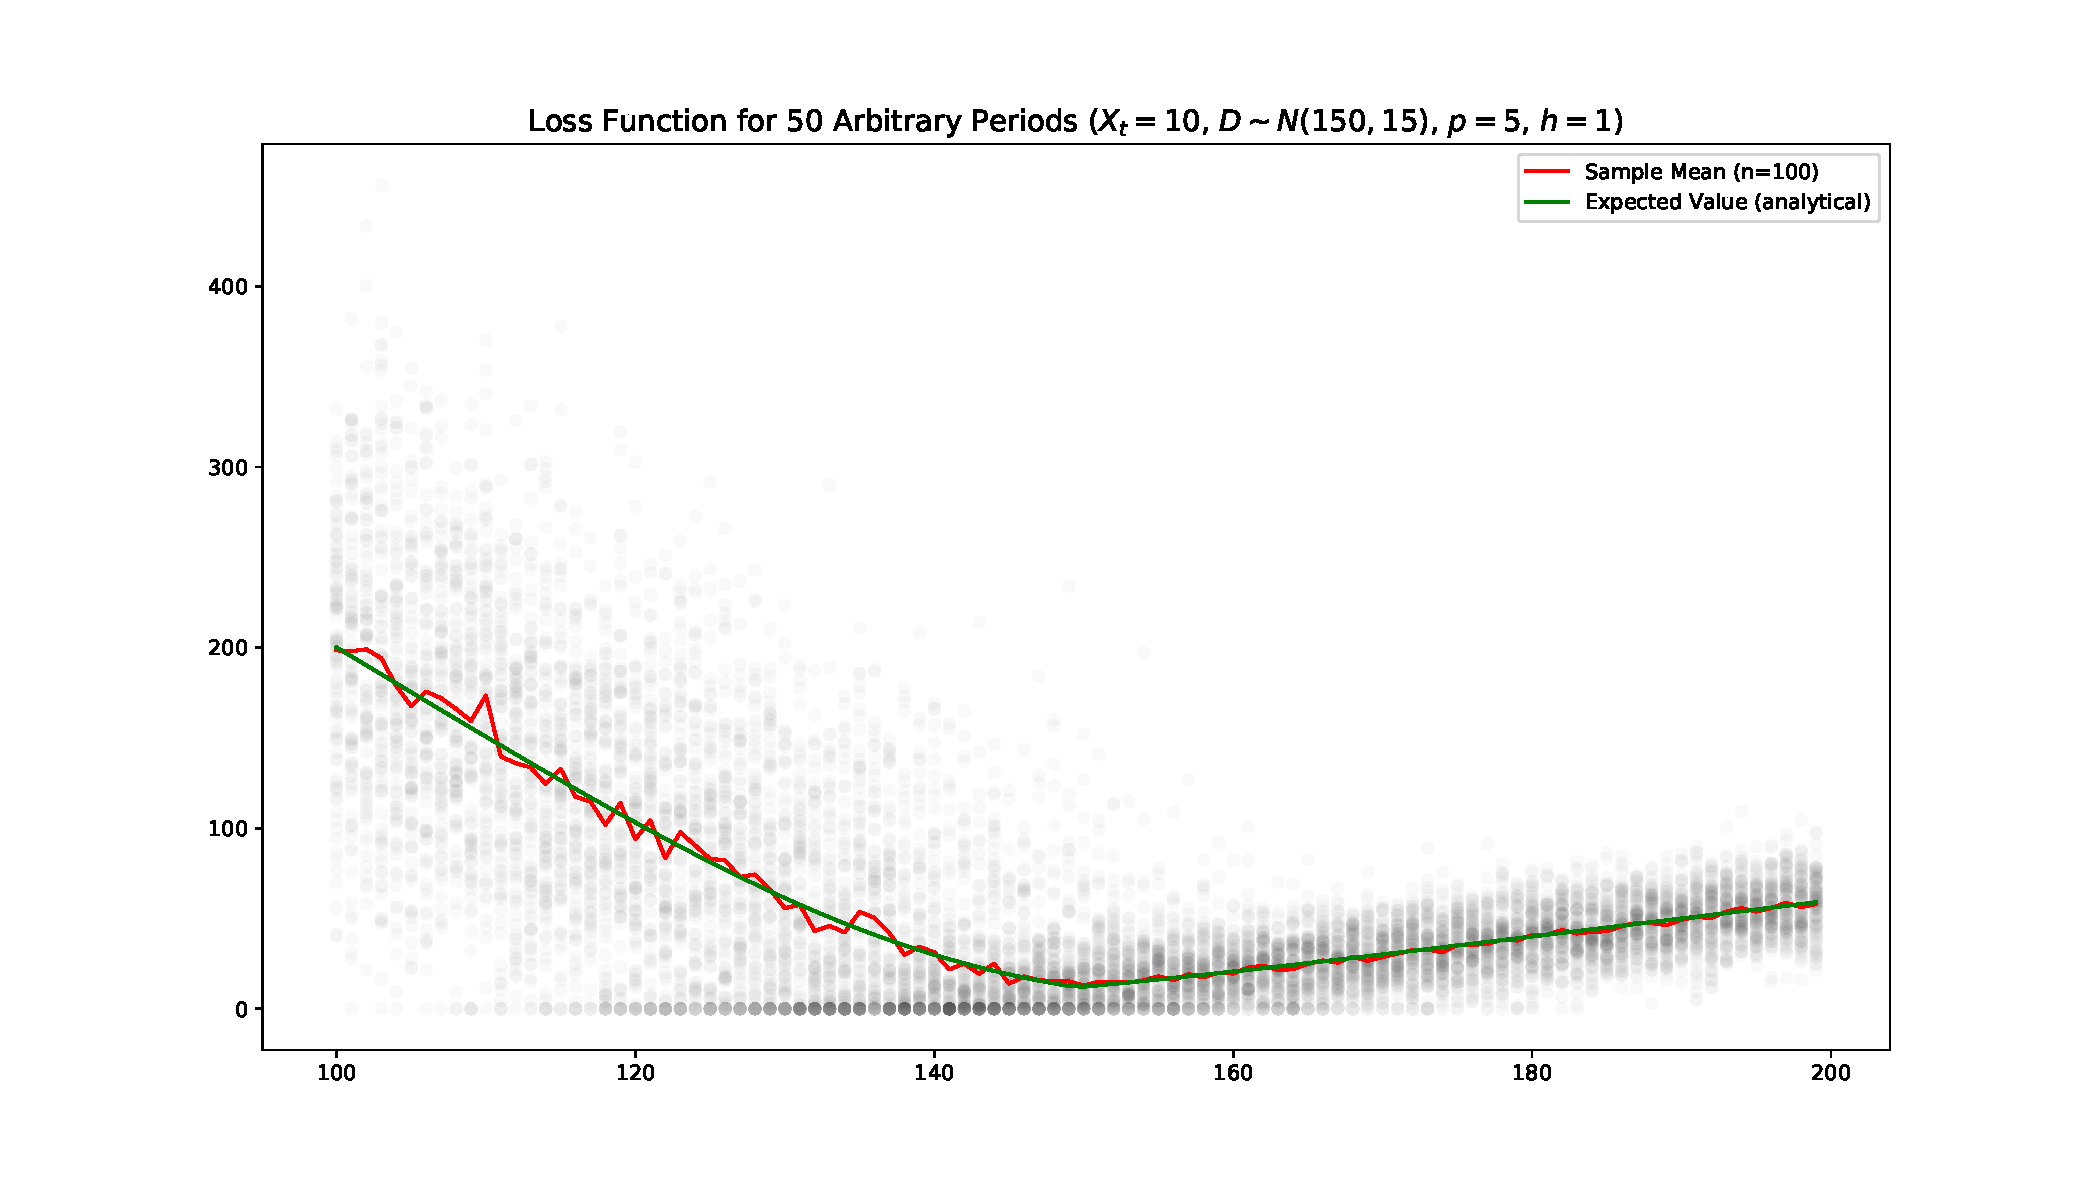
\includegraphics[width=\textwidth]{loss.pdf}

\end{document}